To test the performance of the DataMingler tool we created a set of queries whose execution time was both tested using the tool and traditional data analysis techniques. In particular, we created Jupyter Notebooks that performed the queries using the Python Pandas library and compared the execution time against the DataMingler tool. It is worth noting that apart from performance, the DataMingler tool should be looked at under the scope of ease-of-use and the need for less technical skills to perform queries on multiple data sources. The creation of these notebooks and management of such different data sources is a highly technical and time consuming task. Having a tool that can accelerate the process without any technical knowledge offers many benefits and can save valuable time and resources.

\textbf{Query 1} For each day of the week we want to have the average, minimum, maximum, count and sum of the \texttt{airportFee, driverPay, tripTime, tripMiles, passengerFare} and \texttt{driverTip}. Also we would like to map the \texttt{passengerReviews} to a sentiment score using a sentiment analysis tool to also show the average, minimum, maximum, count and sum of the reviews for each day of the week. A graphical representation of this dataframe query on DVM can be seen in Figure \ref{queryExp1}.

\begin{center}
    \begin{figure}[h]
        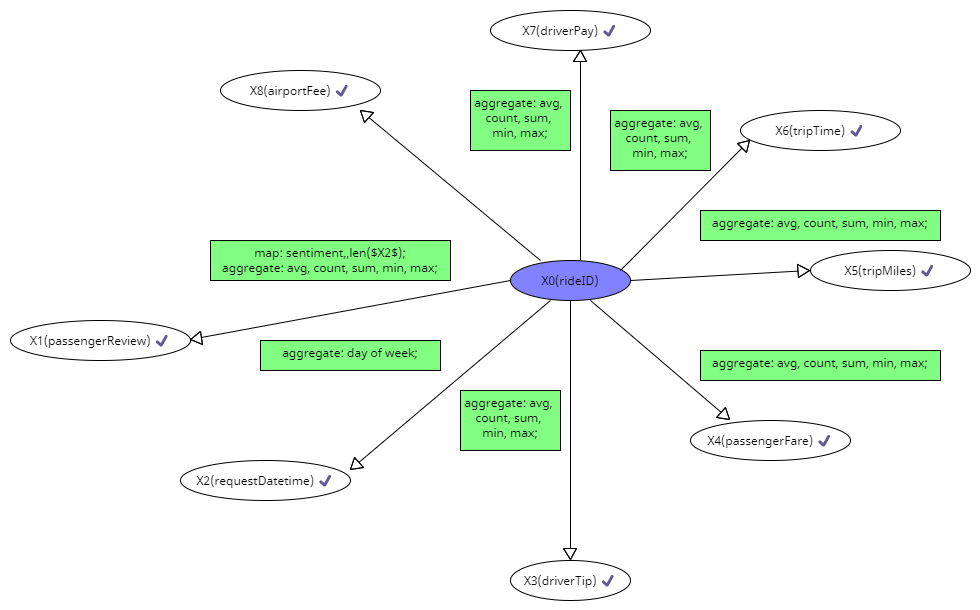
\includegraphics[scale=0.25]{queryExp1}
        \caption{First query of experiment.}
        \label{queryExp1}
    \end{figure}
\end{center}

\textbf{Query 2} For each driver, represented by a unique \texttt{driverUID}, show their \texttt{vehicleModel} and \texttt{gender} along with the average, minimum, maximum, count and sum of their trips \texttt{driverPay, airportFee, passengerReview, driverTip, passengerFare, tripMiles} 
 and \texttt{tripTime}. For the \texttt{passengerReview} the attribute is first going to be mapped using a sentiment analysis tool and then aggregated. A graphical representation of this query on DVM can be seen in Figure \ref{queryExp2}.

\begin{center}
    \begin{figure}[h]
        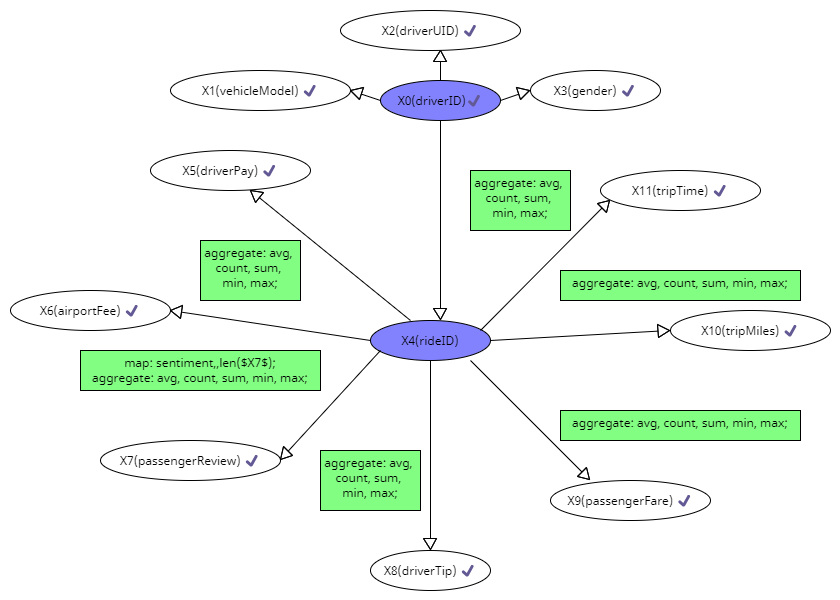
\includegraphics[scale=0.25]{queryExp2}
        \caption{Second query of experiment.}
        \label{queryExp2}
    \end{figure}
\end{center}

\textbf{Query 3} For every location and datetime that taxi trips occurred, represented by \texttt{locationDatetimeID}, show the minimum, maximum, count and sum of the \texttt{airportFee, passengerReview, driverTip, driverPay, passengerFare, tripMiles} and \texttt{tripTime} along with their \texttt{meanCongestion} and \texttt{meanSpeed}. For the \texttt{passengerReview} the attribute is first going to be mapped using a sentiment analysis tool and then aggregated. A graphical representation of this query on DVM can be seen in Figure \ref{queryExp3}.

\begin{center}
    \begin{figure}[h]
        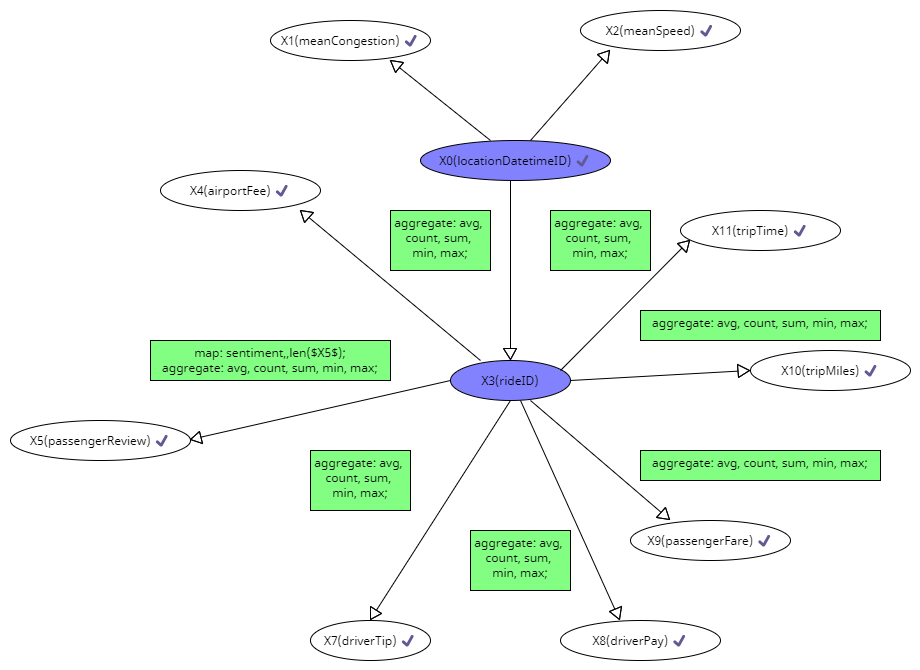
\includegraphics[scale=0.25]{queryExp3}
        \caption{Third query of experiment.}
        \label{queryExp3}
    \end{figure}
\end{center}

\subsection{Algebric evaluation}

\subsection{Optimization}